\documentclass[10pt,twocolumn]{article}
\usepackage[a4paper, left=1.5cm, right=1.5cm, top=2cm, bottom=3cm]{geometry}
\usepackage[T1]{fontenc}
\usepackage[utf8]{inputenc}
\usepackage[italian]{babel}
\usepackage{amsmath}
\usepackage{titling}
\usepackage{caption}
\usepackage{graphicx}
\usepackage{float}
\usepackage{relsize}
\usepackage{amsmath}
\usepackage{sectsty}
\usepackage{ragged2e}
\usepackage{circuitikz}
\usepackage{booktabs}
\usepackage{enumitem}
\usepackage{tikz}
\usepackage{physics}
\usepackage{xcolor}
\usepackage[most]{tcolorbox}
\usepackage{tikz-3dplot}
\usepackage{tikz}
\usepackage{ragged2e}
\usepackage{siunitx}
% \usepackage{booktabs}
\usepackage[colorlinks=true, linkcolor=black]{hyperref}  %per rendere l'indice genrale "interattivo"
\usepackage{enumitem}  %distanza degli itemize
\setlist[itemize]{itemsep=4pt, parsep=1pt}
\newtcolorbox{nota}{
  blanker,
  before skip=1em,
  after skip=1em,
  left=1em,
  borderline west={1pt}{0pt}{black},
  fontupper=\itshape,
  before upper={\noindent\textbf{Nota}:\quad}
}

\begin{document}
\justifying
	\title{\textbf{Misura della costante di Faraday}}
	\author{Brusini Alessio \hspace{0.7cm} Ferrari Carola \hspace{0.7cm} Mirolo Manuele \hspace{0.7cm} Stroili Emanuele}
	\date{28 Ottobre 2025}
	\maketitle
	\newgeometry{left=3cm, right=3cm, top=4cm, bottom=4cm}
	\onecolumn
	\tableofcontents
\vspace{3cm}
	\begin{abstract}
		\centering
		\large
    Lo scopo dell'esperimento è quello di determinare la misura della costante di Faraday tramite una cella elettrolitica costituita da due elettrodi di rame immersi in una soluzione di solfato di rame e acqua.
       
	\end{abstract}

	\newpage
\restoregeometry
\twocolumn

\section{Apparato sperimentale}
Per ottenere la misura a bassi voltaggi si costruisce un circuito composto da:
\begin{itemize}
    \item Generatore di corrente continua
    \item Voltmetro
    \item Amperometro
    \item Becher
    \item Acqua bidistillata
    \item Elettrodi di rame
    \item Solfato di rame
    \item Parallelepipedo di plexiglass
    \item 
\end{itemize}
\begin{figure}[H]
    \centering
    \includegraphics[width=0.5\textwidth]{} % o .png, .pdf, ecc.
    \label{fig:I/V_fotodiodo}
\end{figure}
\section{Procedimento di misura}
La misura si svolge in due fasi: nella prima si prendono misure più fitte
per poter apprezzare le oscillazioni di corrente. A questo scopo è necessario
introdurre una resistenza nel circuito da utilizzare come partitore di tensione.
Inoltre, nella prima fase, ci si serve di un fotodiodo per poter captare la 
flebile luminescenza della lampadina, non visibile univocamente a occhio nudo.\\
Nella seconda fase si prendono dati meno fitti, perciò si rimuovono la 
resistenza e il fotodiodo dal circuito, non più necessari nella misura.

\section{Grafici}
\begin{figure}[H] % [h] = here, posizione approssimativa
  \centering
  %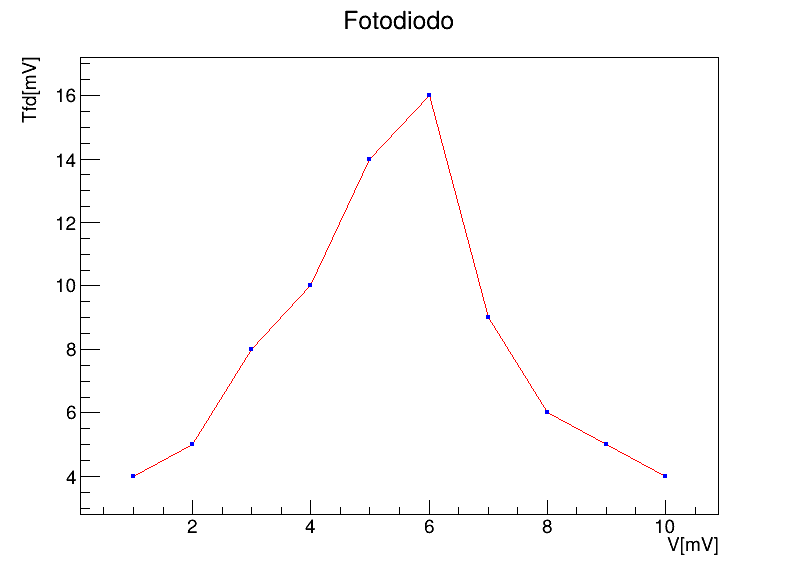
\includegraphics[width=0.5\textwidth]{curva_voltammetrica/fotodiodo.png} % o .png, .pdf, ecc.
  %\label{fig:I/V_fotodiodo}
\end{figure}
Nel grafico si può osservare qual è la differenza di potenziale (V) che va applicata alla lampadina per osservare il primo fenomeno soglia, ovvero l'emissione di fotoni dovuta all'eccitazione degli atomi del tungsteno.
%Nel grafico possiamo osservare a quale differenza di potenziale ai capi della mia lampadina (V) si verifica il primo fenomeno soglia, ovvero l'emissione di fotoni. 
Da quel punto in poi la lampadina non avrà più un comportamento ohmnico. Questo è dovuto al fatto che la forza elettromotrice, oltre alla semplice accelerazione degli elettroni, provoca anche l'agitazione termica del filamento di tungsteno, che inizia a riscaldarsi e quindi a emettere luce visibile, dissipando così energia sotto forma di calore. \\
Essendo questo fenomeno non lineare, la resistenza interna della lampadina non sarà più costante, a partire da quel punto. 


\section{Conclusione}
Non potendo dare una stima quantitativa per stabilire la riuscita
 dell'esperimento è possibile darne una stima qualitativa: osservando 
 il terzo grafico, come già analizzato in precedenza,
  è possibile notare che l'andamento lineare dei valori di corrente misurata in 
  funzione della radice quadrata della tensione stanno ad indicare come la corrente, 
  per la maggior parte dei dati raccolti, in particolare per il range  $400-13000mV$, 
  abbia proprio andamento $I \propto \sqrt{V}$ che ci si aspettava in virtù del fatto
   che la lampadina sottoposta a valori simili di differenza di potenziale non si comporta in modo ohmico

\end{document}